\section{P, NP, and Cook's theorem}
\subsection{NP completeness teori}
\begin{itemize}
  \item Modellen studeret i NP completeness:
  \begin{itemize}
    \item Computeren indeholder bits og bytes. 
    \item Størrelsen af inputtet er antallet af bits i inputtet. 
    \item Tidskompleksitet af en algoritmen er antallet af bit operationer udført.
  \end{itemize}
  \item Problemerne er formuleret som afgørlighedsproblemer 
  \item Inputs er strenge over $\{0,1\}$
  \item Par funktionen $\langle \cdot, \cdot \rangle$ kan bruges til at repræsentere tuples og lister:
  \begin{equation*}
     \langle x, y \rangle = x_1 0 x_2 0 \dots x_{n-1}x_n 011 y_1 0y_20 \dots y_{m-1} 0 y_m 0
  \end{equation*}
  $x$ og $y$ kan hentes ud fra $\langle x, y \rangle$ 
  \item For at få en funktionen $f$ der givet en binær streng giver en binær streng som output kan følgende afgørlighedsproblem $L_f$ defineres:
  \begin{equation*}
    L_f = \{\langle x, b(j), y \mid x \in \{0,1\}^*, j\in N, y \in \{0,1\}, f(x)_j = y \}
  \end{equation*}
  Dette sprog bliver brugt som en stand in for funktion $f$ 
  \item Givet et optimeringsproblem OPT på følgende form: 
  \smallskip

  \textit{``Given en input, som definere et set af løsninger $F$ og en objektiv funktion $f$, find $x \in F$ der maksimere $f(x)$''}
  \item Med et beslutnings problem OPT er der følgende beslutningsproblem $L_\text{OPT}$: 
  \smallskip
  
  \textit{``Given en input streng, som definere et sæt af løsninger $F$, $f$ og en target værdi $v \in \mathbf Q$ beslut hvorvidt der er en løsning $x \in F$ således at $f(x) \geq v$'' } 
  \begin{itemize}
    \item $L_{OPT}$ er brugt som et stand-in for OPT 
    \item Den bliver brugt til at argumentere for at OPT ikke har en effektiv algoritme
  \end{itemize}
  \item \textbf{Church-Turing thesis} Ethvert beslutningsproblem der kan blive løst af en algoritme kan blive løst af en Turing maskine 
\end{itemize}

\subsection{Language complexity}
\begin{itemize}
  \item En Turing afgør et sprog i \textbf{polynomiel tid}, hvis der eksister et fast polynomium $p$, således at antallet af trin taget for ethvert input $x$ er mest $p(|x|)$  
	\item \textbf{Kompleksitetsklassen} $\mathbf P$ er klassen af sprog, der kan blive besluttet i polynomiel tid af en Turing maskine
  \item \textbf{Polynomiel Church-Turing thesis} Et beslutningsproblem kan blive løst i polynomiel tid i et ordenlig sekvensiel model for beregning hvis og kun hvis det kan blive løst i polynomiel tid af en Turing Maskine.
  \item $f:\{0,1\}^* \rightarrow \{0,1\}^*$ er et \textbf{polynomial time computable map}, hvis følgende to egenskaber er overholdt:
  \begin{enumerate}
  	\item Der eksisterer et polynomium $p$, således at $\forall x : |f(x)| \leq p(|x|)$
    \item $L_f \in \mathbf P$, hvor $L_f$ er det beslutningsproblem associerede med $f$
  \end{enumerate}
  \item En repræsentation $\pi$ er \textbf{god} hvis $\pi(S)$ er i $\mathbf P$ 
  \begin{itemize}
  	\item dvs. hvis det kan blive besluttet effektivt hvorvidt en given streng er en korrekt repræsentation af et objekt
  \end{itemize}
  \item To representationer $\pi_1$ og $\pi_2$ er polynomiel ækvivalente hvis der er en polynomiel tid udregnelige maps $r_1$ og $r_2$ der oversætter mellem representationer dvs.:
  \begin{equation*}
    \forall x \in S: \pi_1(x) = r_1(\pi_2(x)) \text{ and } \pi_2 (x) = r_2(\pi_1(x))
  \end{equation*}
	\item \textbf{NP} er klassen af sprog $L$ hvor der eksister et sprog $L' \in \mathbf P$ og et polynomium $p$ således at
  \begin{equation*}
    \forall v: x \in L \Leftrightarrow [\exists y \in \{0,1\}^* : |y| \leq p(|x|) \land \langle x, y \rangle \in L']
  \end{equation*}
  \item Given to sprog $L_1$ og $L_2$ reducerer $L_1$ til $L_2$, hvis der er en polynomiel udregnelig funktion $r$ således at for alle $x \in \{0,1\}^*$ har at
  \begin{equation*}
    x \in L_1 \Leftrightarrow r(x) \in L_2
  \end{equation*}
  Skrevet som $L_1 \leq L_2$ 
  \item \textbf{Proposition} Hvis $L_1 \leq L_2$ og $L_2 \leq L_3$ så gælder $L_1 \leq L_3$
  \item \textbf{Proposition} Hvis $L_1 \leq L_2$ og $L_2 \in \mathbf P$ så gælder der $L_1 \in \mathbf P$
  \item Et sprog $L$ er et $\mathbf{NP}$ hård sprog, hvis den har den egenskab af for alle $L' \in \mathbf{NP}$, $L'$ reducerer til $L$ 
  \item \textbf{Proposition} Lad $L$ være et $\mathbf{NP}$ hårdt sprog. Hvis $\mathbf P \neq \mathbf{NP}$ så gælder der $L \notin P$
  \item Klassen $\mathbf{NPC}$ er klassen af $\mathbf{NP}$ komplette sprog, som er de sprog i NP som er NP hårdt.
  \item \textbf{Proposition} Lad $L \in \mathbf{NPC}$. Så er $\mathbf P = \mathbf{NP}$ hvis og kun hvis $L$ er i $\mathbf P$
\end{itemize}

\subsection{SAT og Circuit SAT}
\begin{itemize}
	\item Et \textbf{boolean circuit} med $n$ input port og $m$ output port er en directed acyclic graph $G=(V,E)$ 
  \begin{itemize}
  	\item Hver knude, kaldes en port og får tildelt et label kan tages fra en af følgende set
    \begin{itemize}
    	\item Funktion symboler: $\{AND, OR, NOT, COPY\}$
		  \item Konstant symboler: $\{0,1\}$
		  \item Variabel symboler: $\{X_1, X_2, \dots, X_n\}$
    \end{itemize}
    \item Alle gates med et variabelt symbol er \textbf{input gates}
    \item Kanterne i grafen kaldes for ledninger
    \item $m$ gates er \textbf{output port}, som bliver kaldt $o_1, o_2, \dots, o_m$
  \end{itemize}
  \item Et Boolean circuit definere en boolean funktion $f:\{0,1\}^n \leftarrow \{0,1\}^m$, som bliver defineret ud fra potenes tilsvarende boolean funktion
  \begin{itemize}
  	\item Dette bliver refereret til som at evaluere circuitet og bliver skrevet på følgende må:
    \begin{equation*}
      C(x) = y
    \end{equation*}
    \item Alle port bliver evalueret siden grafen er en DAG
  \end{itemize}
  \item \textbf{Lemma} For enhver boolean funktion $f: \{0,1\}^n \rightarrow \{0,1\}^m$, eksistere der et $C$, således at $\forall x \in \{0,1\}^n : C(x) = f(x)$
  \item Circuits kan blive brugt som generet udregning enhed
  \begin{itemize}
  	\item Det tager dog kun en fixed input længde modsat TM 
  \end{itemize}
  \item \textbf{Lemma} Lad en TM $M$ som kører i tid højest $p(n) \geq n$ på inputs af længde $n$, hvor $p$ er et polynomium. \smallskip

  Så given enhver input længde $n$, eksistere der et circuit $C_n$ af størrelse $O(p(n)^2)$ således at for alle $x \in \{0,1\}^n$, $C_n(x) = 1$ hvis og kun hvis $M$ acceptere $x$. \smallskip
  
  Funktionen der mappe $1^n$ til en beskrivelse af $C_n$ kører i polynomiel tid. 
  \begin{proof} 
    Siden at TM $M$ kører i tid $p(n)$ kan den kun rører positioner $-p(n), \dots, 0, \dots, p(n)$ under udregning. Enhver anden celle vil aldrig se hoved og vil indeholde det blanke symbol $\#$ under hele udregning. \smallskip

    Definere $c_{t,i}$ for position $i \in \mathbb Z$ og tid $t \in \{0,\dots,p(n)\}$ til at indeholde følgende information:
    \begin{enumerate}
    	\item Det symbol der er i den angivne tape celle på dette tidspunkt
      \item Hvorvidt tapehovedet peger på det punkt på dette tidspunkt
      \item Hvis tape hovedet peget på tapehovedet på dette tidspunkt, tilføjes information omkring tilstanden af den endelig kontrol 
    \end{enumerate}
    Siden $c_{t,i}$ indeholder en endelig mængde information kan den enkodes som en bitstreng $c_{t,i} \in \{0,1\}^s$, hvor $s$ er et tal der kun afhænger af $M$. \smallskip

    Siden $c_{t.i}$ kan udregnes ud fra $c_{t-1,i-1}$, $c_{t-1,i}$ og $c_{t-1,i+1}$ kan følgende funktion defineres $h: \{0,1\}^{3s} \rightarrow \{0,1\}^s$ således at $c_{t,i} = h(c_{t-1,i-1}, c_{t-1,i}  c_{t-1,i+1})$. Siden det vides at alle binær funktioner kan udregnes af en circuit definere vi circuit $D$ til at udregne $h$. \smallskip
    
    Følgende circuit skal også bruges:
    \begin{itemize}
    	\item Et circuit $E$ der udregner $E: \{0,1\} \rightarrow \{0,1\}^s$ således at $E(b)$ er en cell state vektor der repræsenterer en celle der indeholder symbolet $b \in \{0,1\}$ og som ikke indeholder tape hoved. 
    	\item Et circuit $F$ der udregner $F: \{0,1\}^s \rightarrow \{0,1\}$ således at $F(y) = 1$ hvis og kun hvis $y$ er en cell state vektor der repræsenterer en celle der indeholde tape hoved og har en accepting configuration. 
   \end{itemize}
    \begin{figure}[h]
    	\centering
    	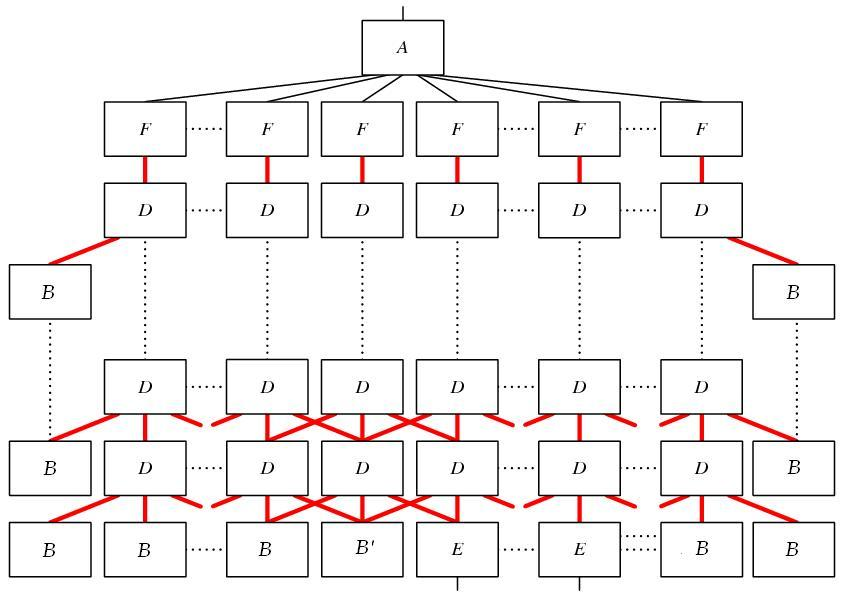
\includegraphics[width=\linewidth]{img/gates_proof}
    	\caption{Circuit $C_n$, hvor de røde linjer repræsenterer ``busses'' der indeholder $s$ ledning \label{gates-proof}}
    \end{figure}
  Siden vi har brug for konstante gates definere samling $B$ af konstante gates $B_i, i, \dots,s$ således at $B_i$ indeholder state $i$ af en cell vektor der repræsenterer den blanke celle uden hoved. \smallskip
  
  Det circuit $C_n$ indeholder $(2p(n)+1)p(n)$ subcircuits $G_{t+i}$, et subcircuit for hver position $i \in \{-p(n), \dots, 0, \dots, p(n)\}$ og for hvert tidspunkt $t \in \{0,1,\dots,p(n)\}$. Subcircuit $G_{t,,i}$ skal udregne state vektoren $c_{t,i}$ og er defineret på følgende måde
  \begin{enumerate}
  	\item For $t=0$ og alle $i$ mellem $1$ og $n$, så er subcircuit $G_{t,i}$ en kopi af $E$, men hvor den enkle input gates er erstattet med en COPY gate der tager sit input fra input gate $X_i$ 
  	\item For $t=0$ og $i=0$ lader vi $G_{0,0}$ være en samling af konstante gates $B'$, som samlet repræsenterer cell state vektoren af en blank celle der indeholder hovedet og hvor den endelige control er i \texttt{start} tilstanden. 
  	\item For $t=0$ og $i \notin \{0,1,\dots,n\}$ lade vi $G_{0,i}$ være en kopi af $B$
  	\item For $t \geq 1$ og et hvert $i$ mellem $-p(n)$ og $p(n)$ er subcircuit $G_{t,i}$ en kopi af $D$ men hvor input gates $X_i$ er erstatte med COPY-gates på følgende måde
    \begin{itemize}
    	\item Hver COPY gate der erstatter input gate $X_i$ $i \in \{1,\dots,s\}$ tager som input den i'te output gate af $G_ {t-1,i-1}$, medmindre $i-1 < -p(n)$ i det tilfælde lader vi gaten tager input $B_i$ 
      \item Hver COPY-gate der erstatter input gate $X_{s+i}$ $i \in \{1,\dots,s\}$ tager som input den ite output gate af $G_{t-1,i}$  
    	\item Hver COPY gate der erstatter input gate $X_{2s+i}$ $i \in \{1,\dots,s\}$ tager som input den i'te output gate af $G_ {t-1,i+1}$, medmindre $i+1 > p(n)$ i det tilfælde lader vi gaten tager input $B_i$ 
    \end{itemize}
  \end{enumerate}
  Der tilføjes $2p(n)+1$ kopi af $F$, med navn $H_{j}$ for $j \in \{-p(n), \dots, p(n)$ til circuit $C_n$ på følgende måde: \smallskip

  Input gate $X_i$ af $H_j$ bliver erstattet af en COPY-gate, der kopier den i'te output gate af subcircuit $G_{p(n),j}$ \smallskip
  
  Et circuit $A$ bliver konstrueret der tager OR af $2p(n)+1$ input hvilket kan blive konstrueret med $2(2p(n)+1)  -1$ binær OR-gates rangeret i et træ. Output gaten bliver sat til outputtet af $A$. Dermed er konstruktionen af $C_n$ færdig og har den ønskede egenskab: Den outputter $1$ hvis og kun hvis Turing Maskinen accepter $x$. 

  \end{proof}
  \item Given et set af symboler, der beskriver boolean variabler:
  \begin{itemize}
  	\item En \textbf{literal} er en variabel er den negation
    \item En \textbf{clause} er en junction af et antal af literaler
  \end{itemize}
  \item En \textbf{conjunctive normal form} (CNF) er en conjunction af et antal af clauses 
  \item En \textbf{disjunctive normal form} (DNF) er en disjunction af et antal af clauses
  \item The \textbf{Satisfiability Problem} (SAT) er følgende decision problem: Given en CNF formula, afgør hvorvidt der er en assignment af sandhed værdier til variablerne der gør at formulaen evaluere til sand
  \begin{itemize}
  	\item En sådan assignment bliver kaldt en \textbf{satisfying assignment} til formelen
  \end{itemize}
  \item \textbf{Cook's Theorem} $\text{SAT} \in \mathsf{NPC}$
  \item \textbf{Circuit SAT} er følgende beslutningsproblem: Given en boolean circuit $C$, er der en vektor $x$ således at $C(x) = 1$
  \item \textbf{Theorem} $\text{CIRCUIT SAT} \in \mathbf{NPC}$
  \begin{proof} 
    CIRCUIT SAT er åbenlyst i $\mathbf{NP}$. Derfor mangles der kun at vise, at det er $\mathbf{NP}$ hårdt. Lad $L$ være et sprog i $\mathbf{NP}$. Der skal vises, at der er en polynomieltids reduktion $r$ således at
    \begin{equation*}
      \forall x : x \in L \Leftrightarrow r(x) \in \text{CIRCUIT SAT}
    \end{equation*}
    Siden $L$ er i $\mathbf{NP}$ ved vi per definition, at der er et sprog $L'$ i $\mathbf{P}$ og et polynomium $p$ således at
    \begin{equation*}
      \forall x: x \in L \Leftrightarrow [\exists y \in \{0,1\}^* : |y| \leq p(|x|) \land \langle x,y \rangle \in L']
    \end{equation*}
    Ud fra dette defineres en reduktion således. Given input $x$, lad $r(x)$ være en beskrivelse af et circuit $C$, dette $C$ kan blive skrevet som en disjunction $C \equiv D_0 \lor D_1, \dots D_{p(|x|)}$. Hvert subcuit $D_i$ skal tage $i$ boolean inputs og evaluere til $1$ på input $y \in \{0,1\}^i$ hvis og kun hvis $\langle x, y \rangle \in L'$. Hvis dette kan lade sig gøre er reduktionen komplet. \smallskip

  Lad subcircuit $D_i$ være defineret på følgende. Lad $M$ være en Turing maskine der afgøre $L'$ i polynomiel tid. Fra en tideligere lemma ved vi at givet en input længde $n$ outputter den et circuit $C_n$ der er satisfiable hvis og kun hvis Turing maskinen acceptere. Vi sætter alle inputs for $x$ til en den $x$ der er givet og erstatter alle de krævede med constant gates i.e. således at kun $y$ er variable. Dermed har vi et korrekt circuit $D_i$. Det følger af Polynomial Church-Turing thesis, at dette er korrekt.

  \end{proof}
  \item \textbf{Proposition} $\text{CIRCUIT SAT} \leq \text{SAT}$
  \begin{proof} 
    Givet et circuit med et enkelt output $C$ skal vi definere en CNF formel $f=r(C)$ således at $f$ har en satisfying assignment hvis og kun hvis $C$ har og således at $r$ er en polynomiel tids udregnelig map. CNF formelen $f$ har en variable for hver $g$ af $C$. Variablen bliver refereret til som $g$. 
    \smallskip

    Clausene i $f$ er defineret på følgende måde: 
    \smallskip

    For hver AND-gate $g$ af $C$, som tager input $h_1$ og $h_2$ tilføjes følgende clauses til $f$, som er det samme som følgende statement $g \Leftrightarrow (h_1 \land h_2)$ altså følgende clauses 
    \begin{equation*}
      (\neg g \lor h_1) \land (\neg g \lor h_2) \land (g \lor \neg h_1 \lor \neg h_2)
    \end{equation*}
    For hver OR-gate $g$ af $C$, som tager input $h_1$ og $h_2$ tilføjes følgende clauses til $f$, som er det samme som følgende statement $g \Leftrightarrow (h_1 \Leftrightarrow h_2)$ altså følgende clauses 
    \begin{equation*}
      (g \lor \neg h_1) \land (g \lor \neg h_2) \land (\neg g \lor h_1 \lor h_2)
    \end{equation*}
    For hver NOT-gate $g$ af $C$, som tager input $h$ tilføjes følgende clauses til $f$, som er det samme som følgende statement $g \Leftrightarrow \neg h$ altså følgende clauses 
    \begin{equation*}
      (g \lor h) \land (\neg g \lor \neg h)
    \end{equation*}
    For hver COPY-gate $g$ af $C$, som tager input $h$ tilføjes følgende clauses til $f$, som er det samme som følgende statement $g \Leftrightarrow h$ altså følgende clauses 
    \begin{equation*}
      (g \lor \neg h) \land (\neg g \lor h)
    \end{equation*}
    For hver konstant gate $g$ af $C$ med label $0$ tilføjes clause $(\neg g)$  
    \smallskip

    For hver konstant gate $g$ af $C$ med label $1$ tilføjes clause $(g)$  
    \smallskip

    For output gaten $g$ af $C$ tilføjes clause $(g)$  
    \smallskip
    
    Funktionen $f$ er en conjunction af alle overstående formulæs. Denne reduktion $r$ kører er polynomiel tid beregnelig og det følger af konstruktionen af de individuelle clauses at reduktionen er korrekt. 

  \end{proof}
\end{itemize}

\newpage
%%% Local Variables:
%%% mode: latex
%%% TeX-master: "optimering-noter"
%%% End:
